\section{Auswertung}
\subsection{Überprüfung der Bragg Bedingung}
Die Messwerte zur Überprüfung der Bragg Bedingung befinden sich in Tabelle \ref{tab:tab1}
\begin{table}[H]
  \centering
  \caption{Messwerte der Wärmepumpe}
  \label{tab:tabe1}
    \begin{tabular}{S S S S S S}
    \toprule
    $ t  \: / \si{\second} $ & $ p_a \: / \si{\bar} $ & $ p_b \: / \si{\bar} $ &
    $ T_1 \: / \si{\kelvin} $ & $ T_2 \: / \si{\kelvin} $ & $ P \: / \: \si{\watt} $\\
    \midrule
    0 & 5.0 & 5.0 & 293.65 & 293.65 & 0 \\
    60 & 4.7 & 6.0 & 294.15 & 293.55 & 115 \\
    120 & 4.4 & 6.4 & 295.15 & 293.15 & 118 \\
    180 & 4.5 & 6.9 & 296.35 & 291.95 & 122 \\
    240 & 4.6 & 7.0 & 297.55 & 290.95 & 125 \\
    300 & 4.6 & 7.0 & 298.85 & 289.95 & 125 \\
    360 & 4.5 & 7.2 & 300.05 & 289.15 & 123 \\
    420 & 4.4 & 7.4 & 301.15 & 288.45 & 123 \\
    480 & 4.3 & 7.8 & 302.35 & 287.65 & 122 \\
    540 & 4.2 & 8.0 & 303.55 & 286.95 & 122 \\
    600 & 4.2 & 8.1 & 304.65 & 286.25 & 121 \\
    660 & 4.1 & 8.3 & 305.75 & 285.55 & 121 \\
    720 & 4.0 & 8.5 & 306.75 & 284.95 & 121 \\
    780 & 4.0 & 8.8 & 307.75 & 284.35 & 121 \\
    840 & 3.9 & 9.0 & 308.75 & 283.75 & 121 \\
    900 & 3.8 & 9.1 & 309.65 & 283.15 & 121 \\
    960 & 3.8 & 9.2 & 310.55 & 282.55 & 122 \\
    1020 & 3.8 & 9.5 & 311.45 & 282.05 & 122 \\
    1080 & 3.7 & 9.8 & 312.25 & 281.55 & 122 \\
    1140 & 3.7 & 10.0 & 313.05 & 281.15 & 122 \\
    1200 & 3.7 & 10.0 & 313.9 & 280.65 & 122 \\
    1260 & 3.6 & 10.2 & 314.65 & 280.25 & 123 \\
    1320 & 3.6 & 10.3 & 315.35 & 279.85 & 123 \\
    1380 & 3.6 & 10.6 & 316.15 & 279.45 & 124 \\
    1440 & 3.6 & 10.8 & 316.85 & 279.15 & 124 \\
    1500 & 3.6 & 11.0 & 317.55 & 278.75 & 124 \\
    1560 & 3.6 & 11.1 & 318.25 & 278.55 & 124 \\
    1620 & 3.6 & 11.2 & 318.95 & 278.25 & 125 \\
    1680 & 3.5 & 11.4 & 319.55 & 277.95 & 125 \\
    1740 & 3.5 & 11.5 & 320.15 & 277.65 & 125 \\
    1800 & 3.5 & 11.7 & 320.75 & 277.45 & 125 \\
    1860 & 3.5 & 11.9 & 321.35 & 277.25 & 125 \\
    1920 & 3.5 & 12.0 & 321.95 & 277.05 & 125 \\
    1980 & 3.5 & 12.1 & 322.45 & 276.95 & 125 \\








      \bottomrule
    \end{tabular}
\end{table}


Hieraus lässt sich ein Maximum von 140 Impulsen pro s bei einem Winkel von 28,2°
ablesen.

\subsection{Emissionsspektrum der Cu-Röntgenröhre}
Die Messwerte des Emissionsspektrums sind in Tabelle \ref{tab:tabe2} abzulesen. In
der Abbildung \ref{fig:plot1} sind sie zudem grafisch dargestellt.
\begin{figure}[H]
  \centering
  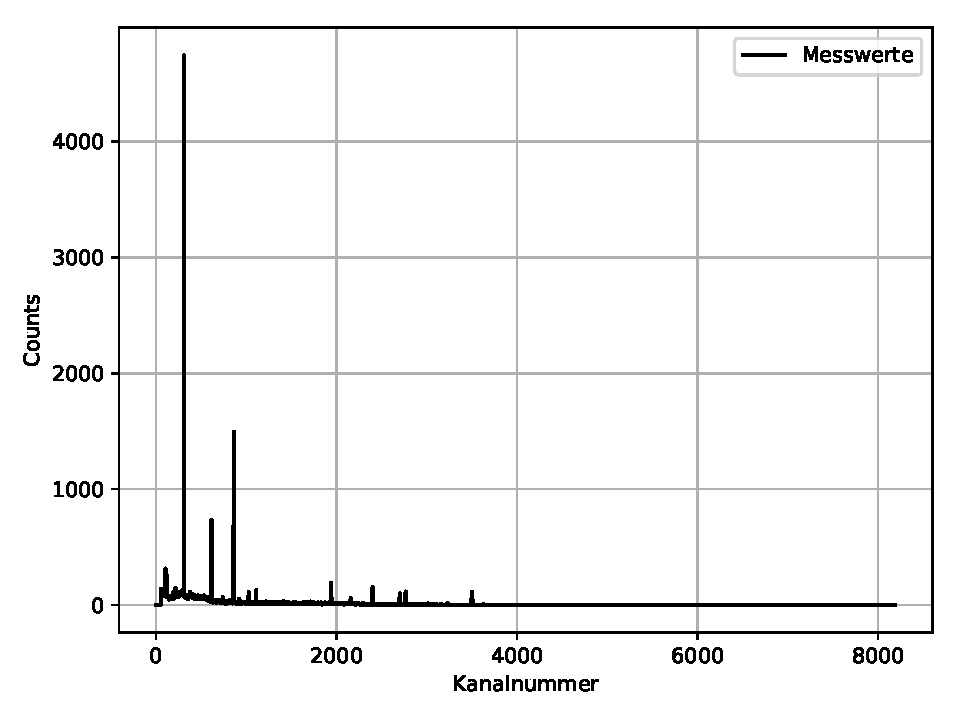
\includegraphics{plot1.pdf}
  \caption{Messwerte des Emissionsspektrums}
  \label{fig:plot1}
\end{figure}
Der Grenzwinkel beträgt hierbei etwa 10°, woraus sich nach Formel \ref{eqn:???} eine minimale
Wellenlänge von $ \SI{35.106}{\pico\meter}$ und eine maximale Energie von $\SI{5.658}{\femto\joule}$
bzw. $\SI{35.317}{\kilo \electronvolt}$ berechen lässt. Die Theoriewerte ergeben sich
aus Gleichung \ref{eqn:???} zu einer minimalen Wellenlänge von $ \SI{35.424}{\pico\meter}$
und einer maximalen Energie von $\SI{5.608}{\femto\joule}$
bzw. $\SI{35}{\kilo \electronvolt}$
Durch die Formel
\begin{equation*}
  \frac{\lvert \text{Wert}_{\text{Theorie}}-\text{Wert}_{\text{Messung}}\rvert}{\text{Wert}_{\text{Theorie}}}
  \label{eqn:abw}
\end{equation*}
ergibt sich somit eine relative Abweichung von $0.9 \%$.

Aus Abbildung \ref{fig:plot1} lässt sich für die Halbwertsbreite der K$\alpha$-Linie
ein Wert von etwa $\Delta \theta$= 0,7° (zwischen 39,70° und 40,40°) ablesen und für die K$\beta$-Linie ein
Wert von etwa $\Delta \theta$= 0,8° (zwischen 44,15° und 44,95°).
Hieraus lässt sich durch $\Delta$E = $\text{E}_1$ - $\text{E}_2$
eine Auflösung von $\SI{0.15}{\kilo\electronvolt}$ (aus K$\alpha$) bzw. $\SI{0.14}{\kilo\electronvolt}$
(aus K$\beta$) berechnen.
Durch die Gleichung
\begin{equation}
  \bar{x} = \frac{1}{N} \sum_{i=1}^{N} x_i \: \:
  \label{eqn:mit}
\end{equation}
\noindent lässt sich der Mittelwert bilden, wobei der dazugehörige Fehler sich durch
\begin{equation}
  \increment \bar{x} = \frac{1}{\sqrt{N}} \sqrt{ \frac{1}{N-1} \sum_{i=1}^N
  (x_i - \bar{x})^2}
  \label{eqn:mitf}
\end{equation}
ergibt.
Somit ergibt sich also insgesamt eine Auflösung von $\SI{0.145(5)}{\kilo\electronvolt}$.


Die Energiedifferenz zwischen der K$\alpha$-Linie und der K$\beta$-Linie beträgt etwa $\SI{0.835}{\kilo\electronvolt}$.
Aus der Gleichung \ref{eqn:???} ergibt sich hieraus eine Abschirmkonstante von



\subsection{Absorptionsspektren}
\subsubsection{Brom}
Die Messwerte des Absorptionsspektrums von Brom sind in Tabelle \ref{tab:tab3} aufgeführt und
in Abbildung \ref{fig:brom} graphisch dargestellt.
\begin{table}
  \centering
  \caption{Messwerte für den ersten Doppelspalt.}
   \begin{tabular}{S S| S S | S S}
    \toprule
    $x/\; \si{\mm}$& $A/\;\si{\nA}$ &
    $x/\; \si{\mm}$& $A/\;\si{\nA}$ &
    $x/\; \si{\mm}$& $A/\;\si{\nA}$ \\
    \midrule

    15.0& 4.6& 23.0& 25.0& 29.5& 6.0\\
    15.5& 4.2& 23.5& 30.0& 30.0& 5.3\\
    16.0& 4.0& 24.0& 35.0& 30.5& 4.9\\
    16.5& 4.0& 24.25& 36.0& 31.0& 4.7\\
    17.0& 4.4& 24.5& 37.0& 31.5& 4.4\\
    17.5& 5.5& 24.75& 38.0& 32.0& 4.2\\
    18.0& 6.6& 25.00& 37.0& 32.5& 3.8\\
    18.5& 7.7& 25.25& 36.0& 33.0& 3.6\\
    19.0& 8.2& 25.5& 36.0& 33.5& 3.2\\
    19.5& 8.4& 26.0& 33.0& 34.0& 3.2\\
    20.0& 8.4& 26.5& 28.5& 34.5& 3.2\\
    20.25& 8.4& 27.0& 23.0& 35.0& 3.3\\
    20.5& 8,7& 27.5& 18.0& 35.5& 3.4\\
    21.0& 9.8& 28.0& 13.5& 36.0& 3.5\\
    21.5& 12.0& 28.5& 10.0\\
    22.0& 15.0& 29.0& 7.8\\
    22.5& 20.0& 29.25& 6.7\\


   \bottomrule
  \end{tabular}
  \label{tab:tabelle3}
\end{table}

\begin{figure}[H]
  \centering
  \includegraphics{Brom.pdf}
  \caption{Absorptionsspektrum von Brom}
  \label{fig:brom}
\end{figure}
Die K-Kante liegt hierbei bei einem Winkel von ungefähr 26,05°, woraus sich nach Formel
\ref{eqn:???} eine Absorptionsenergie von $\SI{13.657}{\kilo}{\electronvolt}$. Durch Gleichung
\ref{eqn:abw} ergibt sich somit eine prozentuale Abweichung von
zum Theoriewert aus der Vorbereitung.


Aus Gleichung \ref{eqn:???} lässt sich aus dieser Absorptionsenergie eine Abschirmkonstante
von ???? berechnen.

\subsubsection{Strontium}
Die Messwerte des Absorptionsspektrums von Strontium sind in Tabelle \ref{tab:tab4} aufgeführt und
in Abbildung \ref{fig:Strontium} graphisch dargestellt.
\begin{table}[H]
  \centering
   \begin{tabular}{c c c c}
    \toprule
    Nummer der Oberwelle & $ U_{\text Theorie,Rechteck}\: / \si{\volt} $ &
    $ U_{\text Theorie,Dreick}\: / \si{\volt} $ & $ U_{\text Theorie,Sägezahn}\: / \si{\volt} $ \\
    \midrule
    1 & 1145 & 182 & 573 \\
    2 & 0 & 0 & 286 \\
    3 & 573 & 20 & 191 \\
    4 & 0 & 0 & 143 \\
    5 & 229 & 7 & 115 \\
    6 & 0 & 0 & 96 \\
    7 & 164 & 4 & 82 \\
    8 & 0 & 0 & 72 \\
    9 & 127 & 2 & 64 \\
    10 & 0 & 0 & 57 \\
    \bottomrule
  \end{tabular}
  \caption{Eingestellte Schwingungsamplituden.}
  \label{tab:tabe4}
\end{table}

\begin{figure}[H]
  \centering
  \includegraphics{Strontium.pdf}
  \caption{Absorptionsspektrum von Strontium}
  \label{fig:Strontium}
\end{figure}
Die K-Kante liegt hierbei bei einem Winkel von etwa 21,70°. Nach analoger Rechnung zu Brom
ergibt sich für Strontium somit eine Absorptionsenergie von $\SI{13.657}{\kilo}{\electronvolt}$
(relative Abweichung: ) und eine Abschirmkonstante von (relative Abweichung: ).

\subsubsection{Zink}
Die Messwerte des Absorptionsspektrums von Zink sind in Tabelle \ref{tab:tab5} aufgeführt und
in Abbildung \ref{fig:Zink} graphisch dargestellt.
\begin{table}[H]
  \centering
  \caption{Bohrung 1 und 2, Vergleich der Sonden mit 1\;MHz und 2\;MHz.}
  \label{tab:tab5}
    \begin{tabular}{c c c c}
    \toprule
    Bohrung & $S_{\text{2\;MHz}}$/\;mm & $S_{\text{ 1\;MHz}}$/\;mm\\
    \midrule
    1 & 1,82 & 2,12\\
    2 & 1,83 & 1,97\\
    \bottomrule
    \end{tabular}
  \end{table}

\begin{figure}[H]
  \centering
  \includegraphics{Zink.pdf}
  \caption{Absorptionsspektrum von Zink}
  \label{fig:Zink}
\end{figure}
Die K-Kante liegt hierbei bei einem Winkel von etwa 36,75°. Nach analoger Rechnung
ergibt sich für Zink somit eine Absorptionsenergie von $\SI{13.657}{\kilo}{\electronvolt}$
(relative Abweichung: ) und eine Abschirmkonstante von (relative Abweichung: ).

\subsubsection{Zirkonium}
Die Messwerte des Absorptionsspektrums von Zirkonium sind in Tabelle \ref{tab:tab6} aufgeführt und
in Abbildung \ref{fig:Zirkonium} graphisch dargestellt.
\begin{table}[H]
  \centering
  \caption{Werte der Anpassungsschicht}
  \label{tab:tabe6}
    \begin{tabular}{S S S }
    \toprule
    $ \text{Zylinder} $ & $ \increment t [\mu\text{s}] $ &
    $ l_a \text{[mm]}$\\
    \midrule
    1 & 0.54 & 0.81 \\
    2 & 0.40 & 0.59 \\
    3 & 0.76 & 1.12 \\
    \text{1+2} & 0.49 & 0.73 \\
    4 & 0.70 & 1.03 \\
    \text{1+3} & 0.90 & 1.33 \\
    5 & 1.25 & 1.85 \\
    \text{1+4} & 0.69 & 1.02 \\
    6 & 0.44 & 0.66 \\

          \bottomrule
    \end{tabular}
  \end{table}

\begin{figure}[H]
  \centering
  \includegraphics{Zirkonium.pdf}
  \caption{Absorptionsspektrum von Zirkonium}
  \label{fig:Zirkonium}
\end{figure}
Die K-Kante liegt hierbei bei einem Winkel von etwa 19,35°. Nach analoger Rechnung
ergibt sich für Zirkonium somit eine Absorptionsenergie von $\SI{13.657}{\kilo}{\electronvolt}$
(relative Abweichung: ) und eine Abschirmkonstante von (relative Abweichung: ).
